\section{三、外文翻译}
\begin{spacing}{1.5}
    \begin{center}
        \zihao{-3}\textbf{硬膜下皮层刺激的研究} \\
        \zihao{4}\textbf{——头部形状、各向异性电导率以及电极形状的影响}\\
        \zihao{-4}$Donghyeon Kim^1,~Hyeon Seo^2,~Hyoung-Ihl Kim^2,~Sung Chan Jun^1$\\
        \zihao{-4}1、信息通讯学院,光州科学技术院,光州,韩国\\
        \zihao{-4}2、医学系统研究所,光州科学技术院,光州,韩国\\
    \end{center}

    \subsection*{摘要}
    \zihao{-4} \hwfs \setlength{\parindent}{2em}
    小四号1.5倍行距,小四号1.5倍行距,小四号1.5倍行距,小四号1.5倍行距,小四号1.5倍行距,小四号1.5倍行距,小四号1.5倍行距,小四号1.5倍行距,
    小四号1.5倍行距,小四号1.5倍行距,小四号1.5倍行距,小四号1.5倍行距,小四号1.5倍行距,小四号1.5倍行距,小四号1.5倍行距,小四号1.5倍行距,    
    \subsection*{简介}

    小四号1.5倍行距,小四号1.5倍行距,小四号1.5倍行距,小四号1.5倍行距,小四号1.5倍行距,小四号1.5倍行距,小四号1.5倍行距,小四号1.5倍行距,
    小四号1.5倍行距,小四号1.5倍行距,小四号1.5倍行距,小四号1.5倍行距,小四号1.5倍行距,小四号1.5倍行距,小四号1.5倍行距,小四号1.5倍行距,
    小四号1.5倍行距,小四号1.5倍行距,小四号1.5倍行距,小四号1.5倍行距,小四号1.5倍行距,小四号1.5倍行距,小四号1.5倍行距,小四号1.5倍行距,
    小四号1.5倍行距,小四号1.5倍行距,小四号1.5倍行距,小四号1.5倍行距,小四号1.5倍行距,小四号1.5倍行距,小四号1.5倍行距,小四号1.5倍行距,


    \begin{figure}[h]
        \begin{center}
        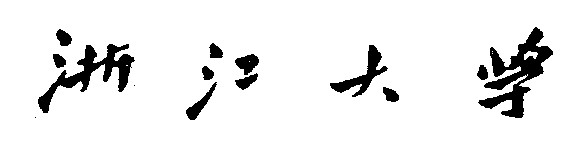
\includegraphics[width=10cm]{ktpics/c1.jpg} 
        \caption{插图示例}
        \end{center}
    \end{figure}
\end{spacing}
\newpage